% 中文摘要      I_chabstract.tex
% 英文摘要      II_enabstract.tex
% 誌謝          III_acknowledge.tex

% 主程式                00_masterthesis.tex
% 緒論                  01_introduction.tex
% 背景知識與相關文獻    02_relatedwork.tex
% 問題分析              03_analysis
% 研究方法              04_method.tex
% 實驗與結果分析        05_experiment.tex
% 結論                  06_conclusion.tex
% 附錄                  07_appendix.tex

% clean.bat 為清除、複製檔案於 C:\xtemp 使用。
% IEEEtran.sty 為文獻格式必須檔。
% *.bib 為文獻檔

%%%%%%%%%%%%%%%%%%%%%%%%%%%%%%%%%%%%%%%%%%%%%%%%%%%%%%%%%%%%%%%%%%%%%%%%%%%%%%%%%%%%%%%%%%%%%%%%%%%%
\documentclass[12pt,oneside,openany,a4paper,draft=FALSE]{book}

% 套件集
%\usepackage[left=3cm,top=3cm,nohead]{geometry}
%\usepackage[total={15cm,24cm}, top=35mm, left=36mm, includefoot]{geometry}
\usepackage[total={15cm,24cm}, top=30mm, left=30mm, includefoot]{geometry}  %版面格式

\usepackage{times}
\usepackage{titlesec}
\usepackage{caption}
\usepackage{comment}
\usepackage{bm}
%\usepackage[usenames,dvipsnames]{color}     %自訂文字顏色
\usepackage{graphicx,subfigure,float}       % 所有圖片均為浮動狀態,可為圖片編碼
\usepackage{amsmath,amssymb}                % 數學式
%\usepackage{color,colortbl,lettrine,wrapfig}
%\usepackage{epstopdf} %EPS轉PDF功能
%\usepackage[bookmarks=false,colorlinks=true,breaklinks=true]{hyperref} %PDF書籤與連結功能
\usepackage[numbered]{bookmark} %PDF書籤與連結功能
\usepackage[titletoc]{appendix}
%\usepackage{breakurl}

% 文獻套件
\usepackage[square,numbers]{natbib} %中英文文獻
%\usepackage{natbib}
\usepackage{bibentry}
%\usepackage{biblatex}
%\usepackage[notocbib]{apacite}     % use APA citation
%\usepackage{IEEEtran}   %IEEE文獻
\usepackage[notindex,nottoc,notlot,notlof]{tocbibind}

\usepackage{longtable}
\usepackage{url}
\usepackage{wallpaper}     % 浮水印

% 表格套件
\usepackage{array}
\usepackage{fancyhdr}
\usepackage{rotating}   % 旋轉表格,將某頁版面由直排轉為橫排,適合用於旋轉占滿一頁的表格或圖形
\usepackage{booktabs}
%\usepackage{graphicx,floatrow}

% 數學
\usepackage{amsthm}     % 排版數學文稿的定理與定義
\usepackage{amsmath}
\usepackage{enumerate}  % 條列項目 (阿拉伯數字編號)

%% 中文專用
\usepackage{fontspec} %加這個就可以設定字體
\usepackage{xeCJK} %讓中英文字體分開設置

%-----

% 設定『目錄』名稱
\renewcommand{\contentsname}{目錄}
\renewcommand{\listfigurename}{圖目錄}
\renewcommand{\listtablename}{表目錄}
%\renewcommand{\appendixtocname}{附錄}   % if \appendix  is used.
\renewcommand{\appendixname}{附錄}   % if \appendix  is used.
\renewcommand{\tablename}{表}
\renewcommand{\figurename}{圖}
\renewcommand{\bibname}{參考文獻}

\hypersetup{
    bookmarks=true,         % show bookmarks bar?
    colorlinks=true,        % false: boxed links; true: colored links
    linkcolor=black,          % color of internal links (change box color with linkbordercolor)
    citecolor=black,          % color of links to bibliography
    filecolor=cyan,         % color of file links
    urlcolor=magenta        % color of external links
}

%\newcommand{\img}{C:/Dropbox/ntpu_thesis/plot/}%如果所有圖檔存放在其他地方,先定義位置

\pagestyle{fancy}
\fancyhf{}
\renewcommand{\chaptermark}[1]{\markboth{\thechapter .\ #1}{}}  % 去除章編號前後的字
\titleformat{\chapter}[display]{\center\LARGE\sf}{第\ \thechapter\ 章}{0.2cm}{}  %設計章節標題式樣,標題置中
\titlespacing{\chapter}{0pt}{-50pt}{25pt}   %設計章節標題式樣,控制間距
%\fancyhead[RO,RE]{\leftmark}   %章節標題於頁眉/頁足上
\fancyfoot[CO,CE]{\thepage}

\renewcommand{\headrulewidth}{0pt}  % 頁眉下方的橫線
%\renewcommand{\footrulewidth}{0pt} % 設定頁首多一條粗細是 0.4 pt 的水平線

% 設定itemize符號
\renewcommand{\labelitemi}{$\bullet$}
\renewcommand{\labelitemii}{$\circ$}

%設定英文字型,不設的話就會使用預設的字型
\setmainfont{Times New Roman}

% 設定中文字體
\setCJKmainfont{標楷體} %設定中文為系統上的字型,而英文不去更動,使用原TeX字型
%\setCJKmainfont{cwTeXKai}
\XeTeXlinebreaklocale "zh"
\XeTeXlinebreakskip = 0pt plus 1pt %這兩行一定要加,中文才能自動換行


\renewcommand{\baselinestretch}{1.25}   %依照文章預設行距增加為 1.25倍(不同字型大小行距值,加大為1.25倍)

% 以下是目錄章節後面打點格式的設定:http://vardesa.blog.hexun.com.tw/58537832_d.html
\makeatletter
\def\@bfdottedtocline#1#2#3#4#5{%
\ifnum #1>\c@tocdepth \else
\vskip \z@ \@plus.2\p@
{\leftskip #2\relax \rightskip \@tocrmarg \parfillskip -\rightskip
\parindent #2\relax\@afterindenttrue
\interlinepenalty\@M
\leavevmode \bfseries
\@tempdima #3\relax
\advance\leftskip \@tempdima \null\nobreak\hskip -\leftskip
{#4}\normalfont\nobreak
\leaders\hbox{$\m@th
\mkern \@dotsep mu\hbox{.}\mkern \@dotsep
mu$}\hfill
\nobreak
\hb@xt@\@pnumwidth{\hfil\normalfont \normalcolor #5}%
\par}%
\fi}
\renewcommand*\l@chapter{\@bfdottedtocline{0}{0em}{1.5em}}
\makeatother

% 定義『各章節標題、圖表、頁尾註記』字型

\theoremstyle{plain}   % 排版格式,{plain}:最醒目格式
\newtheorem{thm}{定理}  % 將 Theorem 改為國字「定理」
\newtheorem{thmm}{定義}


%
%   調整內縮長度(依據學校規定與不同版面、字型調整)
%
\parindent=0.85cm
%% 修改中文標題與格式定義
\date{2013.9.18}    %版本日期

%%%%% 論文開始 %%%%%
\begin{document}

%%  封面
%% 封面頁
\fontsize{24}{20pt}\selectfont
\thispagestyle{empty}


\vspace*{1cm}

\vspace*{\fill}
\begin{center}
	\fontsize{24}{18pt}
	%\LARGE 筆記 \\

\end{center}
\vspace*{\fill}



\vspace*{0.5cm}

\begin{center}
	\fontsize{24}{18pt}
	\LARGE 作者:X X X   撰\\
\end{center}

\vspace*{0.5cm}


\newpage


%%
%%\CenterWallPaper{0.17}{graphs/logo/logowatermark.eps} %浮水印
%===============================================================
%%%%%%%%%%%%%%%%---------- 中文摘要
\frontmatter % 羅馬文頁碼


%%  目錄
\newpage
%%\newpage
\fontsize{12}{18pt}\selectfont
%%  目錄
\phantomsection
\addcontentsline{toc}{chapter}{目錄} %手動加入目錄文字
\tableofcontents
\newpage
%%  圖目錄
%%\phantomsection
%%\addcontentsline{toc}{chapter}{圖目錄} %手動加入目錄文字
%%\listoffigures
%%\newpage
%%%%  表目錄
%%\phantomsection
%%\addcontentsline{toc}{chapter}{表目錄} %手動加入目錄文字
%%\listoftables
%%\newpage


%%%%%%%%%%%%%%%%%%%% 碩士論文內文開始 %%%%%%%%%%%%%%%%%%%%

%%%%%%%%%%%%%%%%---------- 開始章節
\cleardoublepage
\mainmatter % 阿拉伯文頁碼
\fontsize{12}{21pt}\selectfont

%%  第一章
\chapter{緒論}
\label{chapter:intro}
\section{研究背景與動機}
\label{sec:background}
    \subsection{子章節一}
        字章節一段落一,字章節一段落一,字章節一段落一,字章節一段落一,
        字章節一段落一,字章節一段落一,字章節一段落一,字章節一段落一,
        字章節一段落一,字章節一段落一,字章節一段落一,字章節一段落一,
        字章節一段落一,字章節一段落一,字章節一段落一,字章節一段落一,
        字章節一段落一,字章節一段落一,字章節一段落一。

        字章節一段落二,字章節一段落二,字章節一段落二,字章節一段落二,
        字章節一段落二,字章節一段落二,字章節一段落二,字章節一段落二,
        字章節一段落二,字章節一段落二,字章節一段落二,字章節一段落二,
        字章節一段落二,字章節一段落二,字章節一段落二,字章節一段落二,
        字章節一段落二,字章節一段落二,字章節一段落二,字章節一段落二,
        字章節一段落二,字章節一段落二,字章節一段落二,字章節一段落二,
        字章節一段落二。

        例如現有的系統有\cite{GoogleComputeEngine}、\cite{AmazonEC2}等等,
        另外\cite{GoogleApps}是以○○○技術來達成。

        ○○系統結構如示意圖\ref{fig:this_system}
        \begin{figure}[htbp]
            \centerline{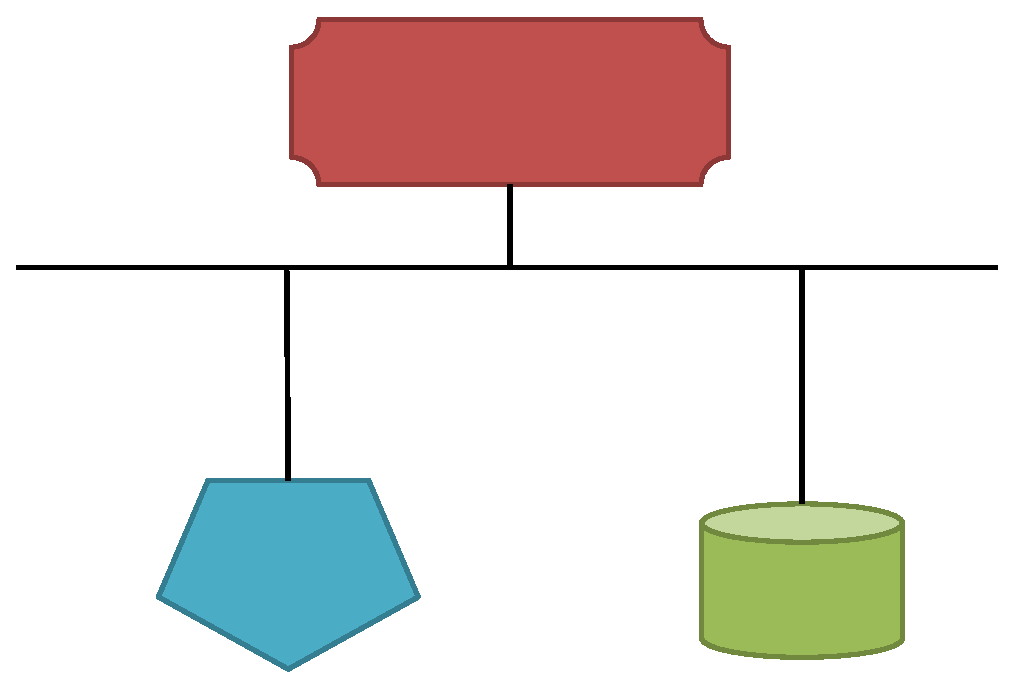
\includegraphics[height=5cm]{graphs/introduction/this_system.eps}}
            \caption{○○示意圖}
            \label{fig:this_system}
        \end{figure}

    \subsection{子章節二}
        字章節二,字章節二,字章節二,字章節二,字章節二,
        字章節二,字章節二,字章節二,字章節二,字章節二,
        字章節二,字章節二,字章節二,字章節二,字章節二,
        字章節二,字章節二,字章節二,字章節二,字章節二,
        字章節二,字章節二,字章節二,字章節二,字章節二,
        字章節二,字章節二,字章節二,字章節二,
        ○○○如圖~\ref{fig:types_comparison}所示。
        \begin{figure}[!t]
            \begin{center}
                \begin{tabular}{ccccccccccccc}
                    \subfigure[類型A]{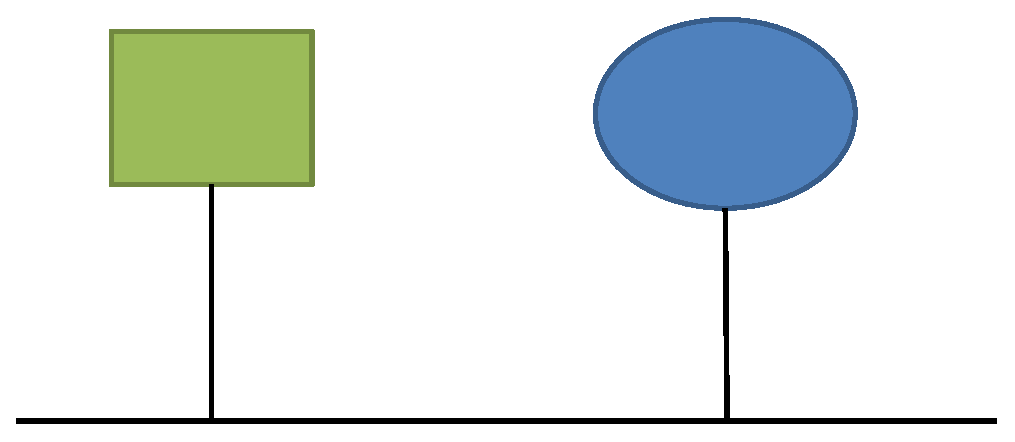
\includegraphics[height=2.4cm]{graphs/introduction/typeA.eps}\label{fig:typeA} } \par &
                    \subfigure[類型B]{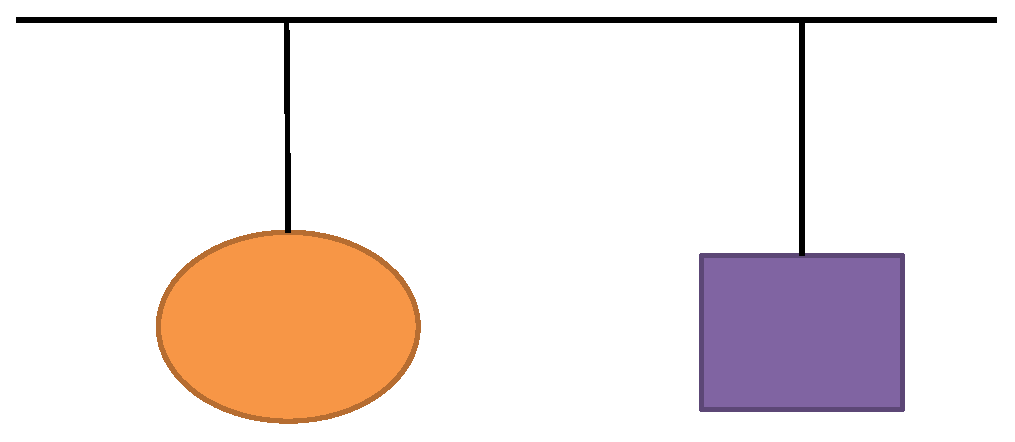
\includegraphics[height=2.4cm]{graphs/introduction/typeB.eps}\label{fig:typeA} } \par \\
                \end{tabular}
                \caption{○○○比較}
                \label{fig:types_comparison}
            \end{center}
        \end{figure}

\section{○○○問題與處理機制}
    問題與機制,問題與機制,問題與機制,問題與機制,
    問題與機制,問題與機制,問題與機制,問題與機制,
    問題與機制,問題與機制,問題與機制,問題與機制,
    問題與機制,問題與機制,問題與機制,問題與機制,
    問題與機制。

    %要被單行註解的文字。

\begin{comment}
    要被區塊註解的文字,要被區塊註解的文字,要被區塊註解的文字,
    要被區塊註解的文字,要被區塊註解的文字,要被區塊註解的文字,
    要被區塊註解的文字,要被區塊註解的文字,要被區塊註解的文字,
    要被區塊註解的文字,要被區塊註解的文字,要被區塊註解的文字,
    要被區塊註解的文字,要被區塊註解的文字,要被區塊註解的文字,
    要被區塊註解的文字,要被區塊註解的文字。
\end{comment}

\section{研究動機與目的}
    動機與目的,動機與目的,動機與目的,動機與目的,
    動機與目的,動機與目的,動機與目的,動機與目的,
    動機與目的,動機與目的,動機與目的,動機與目的,
    動機與目的,動機與目的,動機與目的,動機與目的,
    動機與目的,動機與目的,動機與目的,
    細節如表\ref{tab:mytitle1}。
    \begin{table}[!t]
        \centering
        \caption{表格標題1}
        \label{tab:mytitle1}
        % Table generated by Excel2LaTeX from sheet 'table_01'
\begin{tabular}{rr}
\toprule
Title & Values \\
\midrule
A     & 1612 \\
B     & 256 \\
C     & 30 \\
D     & 7 \\
E     & 3 \\
\bottomrule
\end{tabular}%

    \end{table}

    \begin{enumerate}
        \item
        列舉一。
        %
        \item
        列舉二。
        %
        \item
        列舉三。
        %
    \end{enumerate}

\section {研究方法與論文架構}
    研究方法與論文架構,研究方法與論文架構,研究方法與論文架構,
    研究方法與論文架構,研究方法與論文架構,研究方法與論文架構,
    研究方法與論文架構,研究方法與論文架構,研究方法與論文架構,
    研究方法與論文架構。

    \begin{itemize}
        \item
        項目一。
        %
        \item
        項目二。
        %
        \item
        項目三。
        %
        \item
        項目四。
    \end{itemize}

    流程圖如\ref{fig:ResearchFlowChart}。
    \begin{figure}[htbp]
        \centering
        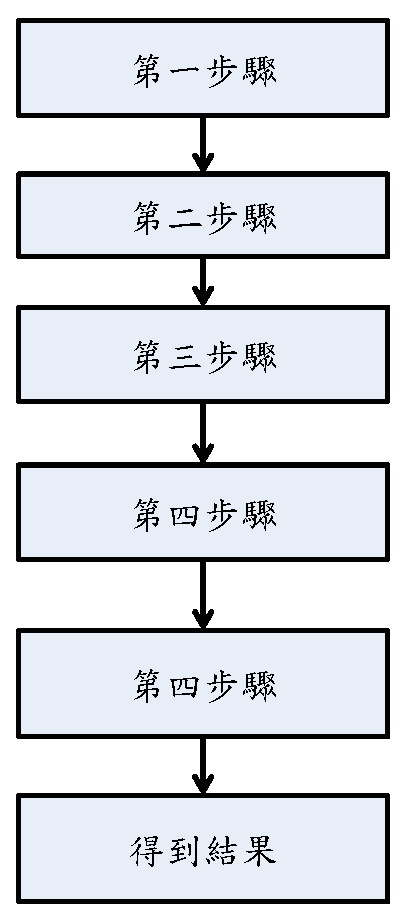
\includegraphics[height=8cm]{graphs/introduction/ResearchFlowChart.eps}
        \caption{研究進行流程圖}
        \label{fig:ResearchFlowChart}
    \end{figure}




%%  文獻
\bibliographystyle{IEEEtran}
%    \bibliographystyle{plain}
%    \bibliographystyle{apa}
%    \bibliographystyle{apacite}\renewcommand{\bibname}{參考文獻}
\bibliography{citations/ref_title1,citations/ref_title2}

%%%%%%%%%%%%%%%%---------- 附錄
\begin{appendices}
	\appendix
	%        \noappendicestocpagenum
	\titleformat{\chapter}[display]{\center\LARGE\sf}{附錄 \thechapter}{0.2cm}{}  % 設計附錄標題式樣,標題置中
	\chapter{相關公式}
\label{chapter:appendix_eq}

    質能互換公式為\eqref{eq:mass_energy_equivalence}。
    \begin{equation}\label{eq:mass_energy_equivalence}
      E=MC^2
    \end{equation}

 %% appendix-A
	\chapter{相關表格}
\label{chapter:appendix_tables}

    ○○○對應表為\ref{tab:mytitle2}。
    \begin{table}[htbp]
        \centering
        \caption{表格標題2}
        \label{tab:mytitle2}
        % Table generated by Excel2LaTeX from sheet '工作表1'
\begin{tabular}{rrr}
\toprule
Number & Class & Values \\
\midrule
1     & A     & 21 \\
2     & B     & 854 \\
3     & C     & 458 \\
4     & D     & 87 \\
5     & E     & 1654 \\
6     & F     & 978 \\
7     & G     & 23 \\
8     & H     & 746 \\
9     & I     & 278 \\
\bottomrule
\end{tabular}%

    \end{table}

 %% appendix-A
\end{appendices}

%===============================================================
\end{document}
